\documentclass[lang=cn]{elegantpaper}

\title{十二月过程性研究记录}
\author{陶理}
\usepackage{listings}
\begin{document}
\date{December 28, 2023}
\maketitle

\begin{abstract}
    该份过程性研究记录(截止至撰写日期)主要记录了作者在十二月所完成的研究成果。主要有以下几项:
    \begin{enumerate}
        \item 对普通话的语音指令数据进行进一步处理:如能量分布和MFCCs等特征
        \item 对处理后的数据进行分析
    \end{enumerate}
\end{abstract}

\section{普通话语音指令数据的处理和特征提取}
\subsection{数据收集}
还是采用了和11月份一样的数据(22条普通话语音指令)
\subsection{能量分布}
一段音频的能量分布能够对于语音识别起到一定作用,因此对它进行分析。
下面是我对目前所有22条数据进行能量分布曲线的绘制,结果如下:
\begin{figure}[h]
    \centering
    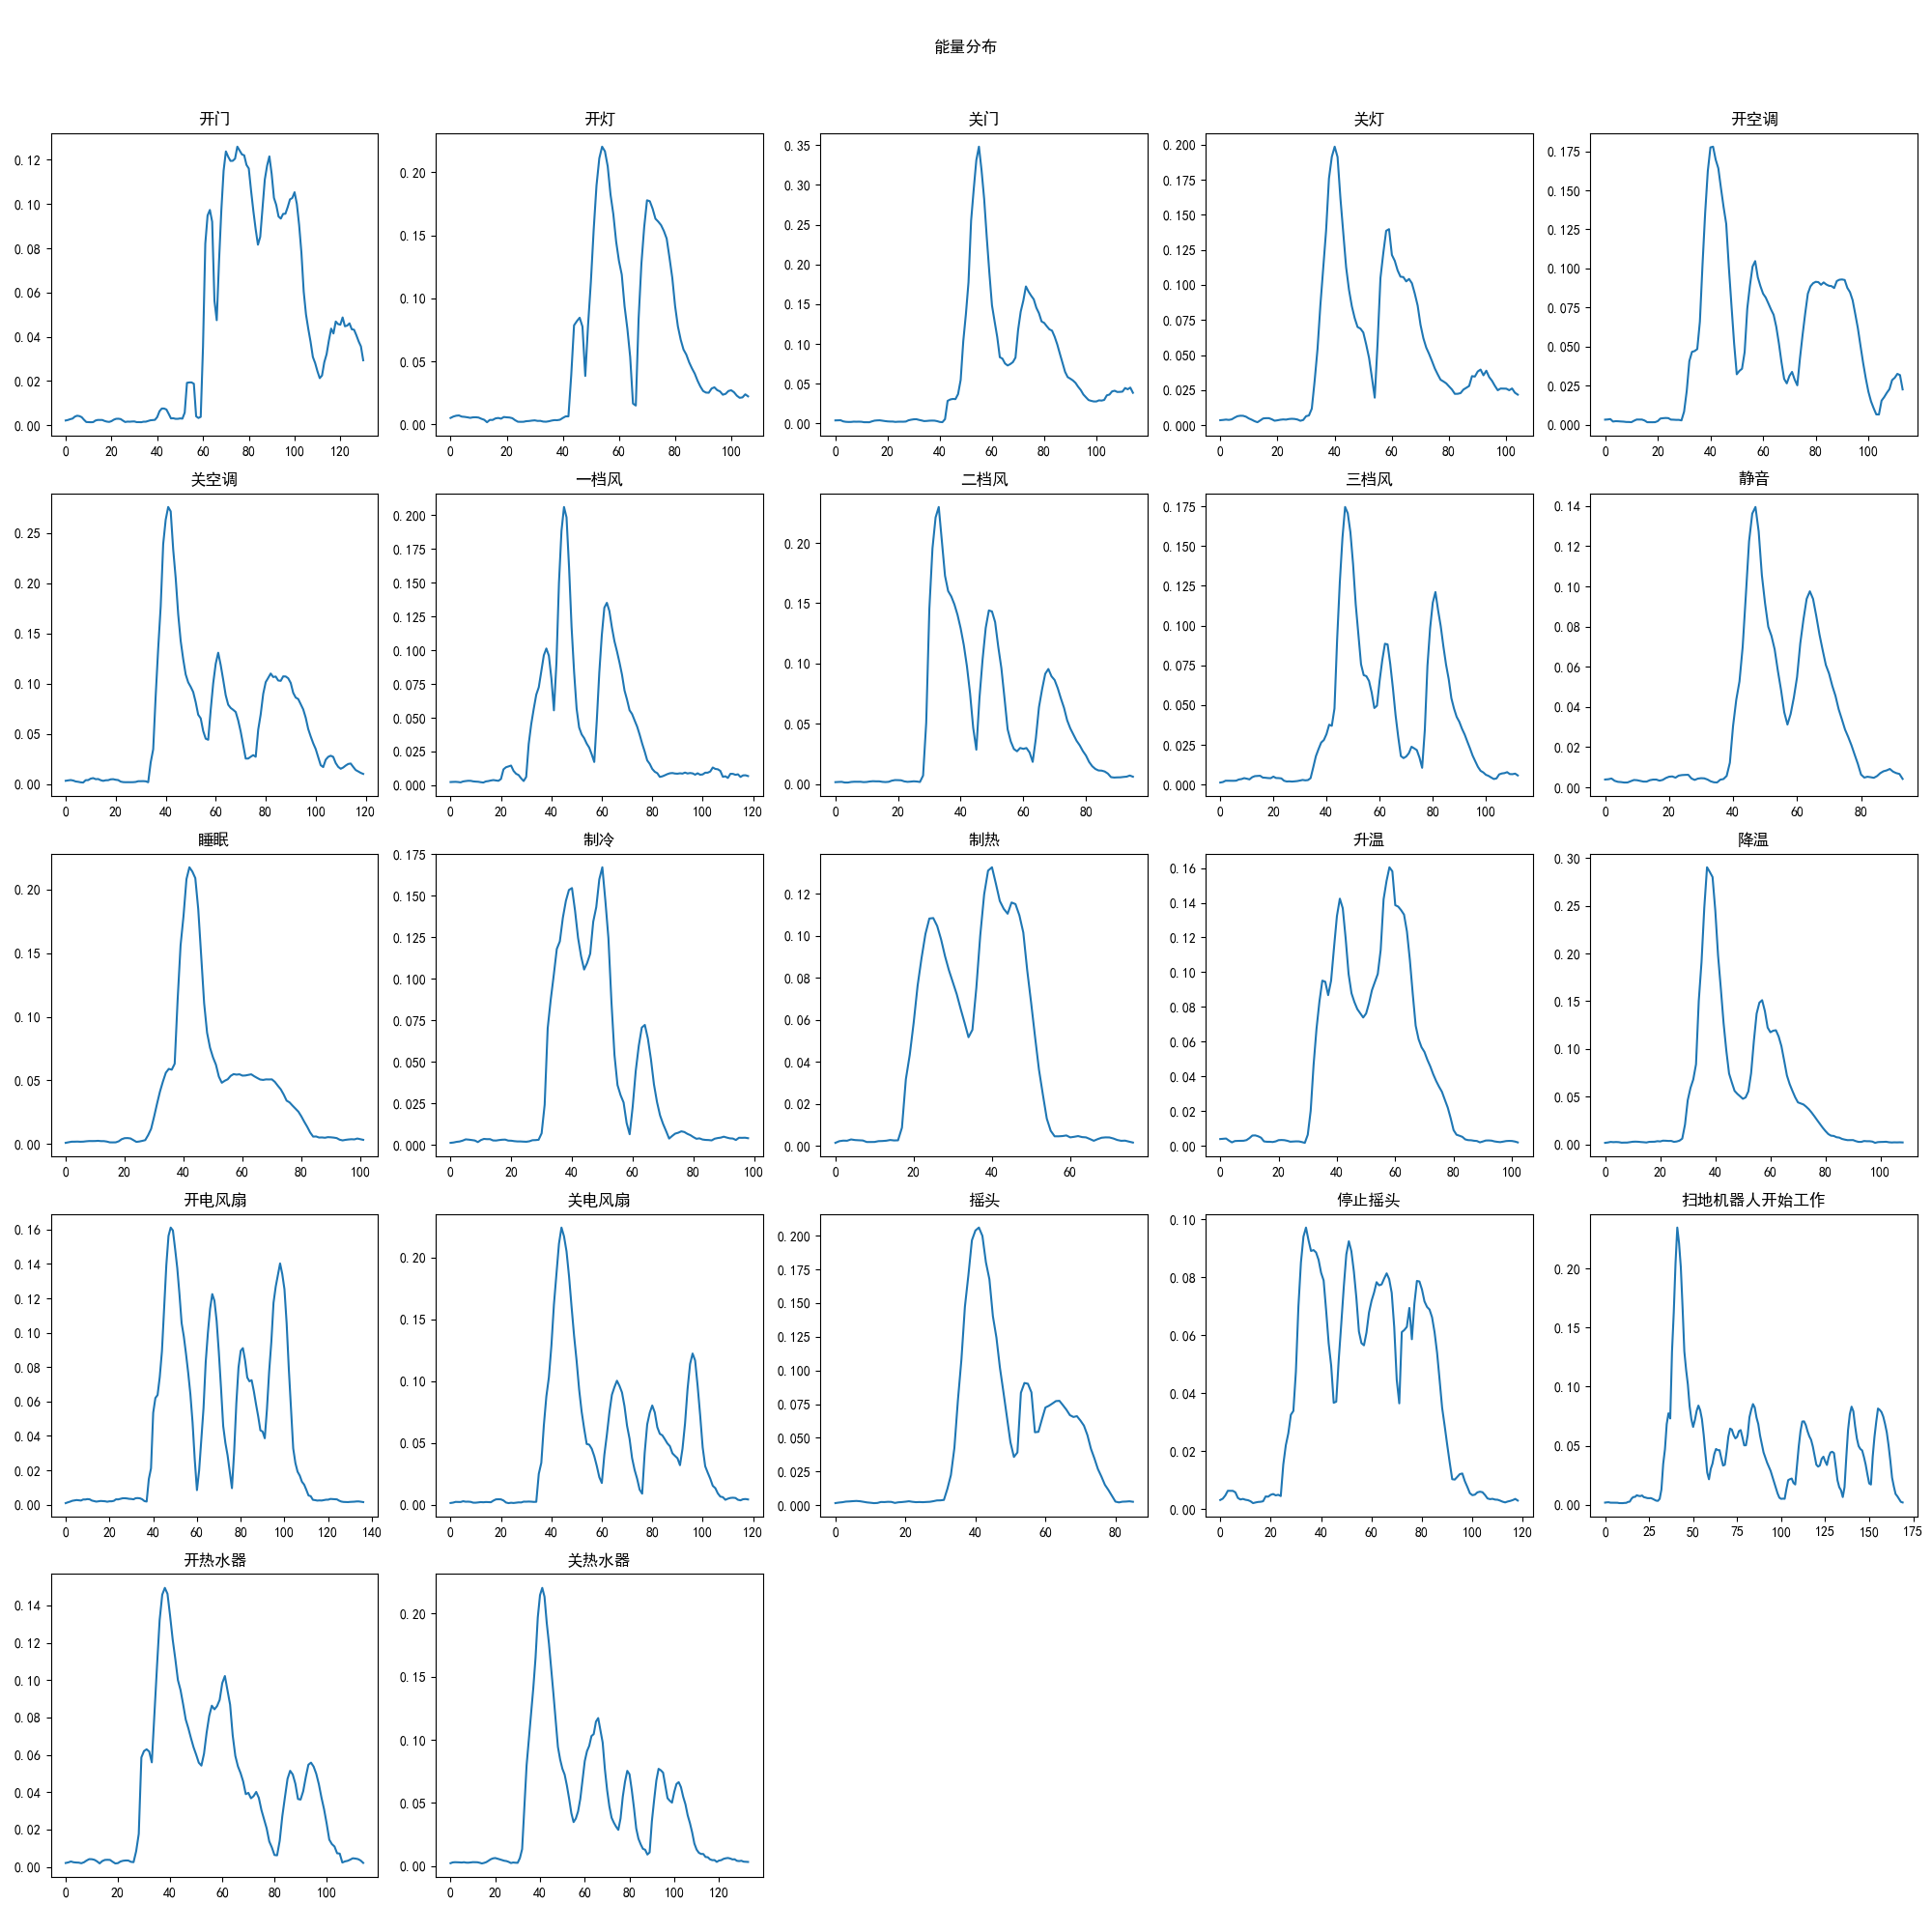
\includegraphics[width=0.59\textwidth]{energydistribution.png}
\end{figure}

程序如下:
\begin{lstlisting}[language=Python]
import os
import librosa
import librosa.display
import matplotlib.pyplot as plt
import math
plt.rcParams['font.sans-serif'] = ['SimHei']
def generate_energy_distribution(audio_file, label):
    y, sr = librosa.load(audio_file)
    energy = librosa.feature.rms(y=y)
    return energy, label
energy_data = []
labels = ['...','...',...,'...']
for i in range(1, 23):
    audio_file = '...'
    energy, label = generate_energy_distribution(audio_file, labels[i-1])
    energy_data.append((energy, label))
num_images = len(energy_data)
num_cols = 5
num_rows = math.ceil(num_images / num_cols)
fig, axes = plt.subplots(nrows=num_rows, ncols=num_cols, figsize=(20, 20))
for i in range(num_images):
    row = i // num_cols
    col = i % num_cols
    ax = axes[row, col]
    ax.plot(energy_data[i][0][0])
    ax.set_title(f'{energy_data[i][1]}')
for i in range(num_images, num_rows * num_cols):
    fig.delaxes(axes.flatten()[i])
plt.tight_layout(rect=[0, 0.01, 1, 0.95])
plt.suptitle('...')
plt.savefig('...')
plt.show()
\end{lstlisting}
\subsection{MFCC}
\textbf{定义}:梅尔频率倒谱系数 (Mel-Frequency Cepstral Coefficients,MFCCs)就是组成梅尔频率倒谱的系数。它衍生自音讯片段的倒频谱 (cepstrum)。
倒谱和梅尔频率倒谱的区别在于,梅尔频率倒谱的频带划分是在梅尔刻度上等距划分的,它比用于正常的对数倒频谱中的线性间隔的频带更能近似人类的听觉系统。 (\textit{源自维基百科}) 

以下是计算mfccs的Python程序:
\begin{lstlisting}[language=Python]
import librosa
import numpy as np
def extract_mfcc(file_path):
    y, sr = librosa.load(file_path)
    mfccs = librosa.feature.mfcc(y=y, sr=sr, n_mfcc=13)
    return mfccs
mfcc_data = []
for i in range(1, 23):
    file_path = f'...'
    mfccs = extract_mfcc(file_path)
    mfcc_data.append(mfccs)
print(mfcc_data)
\end{lstlisting}
\end{document}